Correlation analysis is a ubiquitous problem in statistical signal processing. In many
applications, we have access to multiple datasets each using a different feature space to
describe a system. In image annotation \cite{hardoon2006correlation} and image retrieval
\cite{hardoon2004canonical} we assume that both image features and textual captions
describe the depicted scene. In speaker identification, we assume that the video of a
speaker is correlated with his/her audio \cite{chaudhuri2009multi}.  In medical signal
processing, we assume that different modalities such as EEG, MEG, MRI, fMRI, and genetic
data (SNPs, QTs) capture a shared signal of interest in a patient
\cite{deleus2011functional,correa2010canonical,wilms2013sparse,zhang2013l1,
singanamalli2014supervised,yan2014accelerating,spuler2013spatial,
lin2014correspondence,campi2013non}.  With the increasing ability to collect such a
variety of data, multimodal datasets even make appearances in non-classical statistical
signal processing applications such as economics \cite{todros2012measure,doscanonical},
climatology \cite{wilks2014probabilistic,prera2014using}, and psychology
\cite{vilsaint2013ecology,travis2014creativity}.

In many of these applications, we model observations using a low rank signal-plus-noise
model. This model assumes that observations from a dataset lie in an unknown low-rank
subspace and that the signal vectors between datasets are correlated. We obtain estimates
of the unknown signal subspace and signal-to-noise ratios (SNR) of signals in a particular
dataset via the eigenvalue decomposition of its sample covariance matrix. The accuracy of
this eigenvalue decomposition has been extensively studied
\cite{paul2007asymptotics,benaych2011eigenvalues} and applied to applications such as
matched subspace detection \cite{asendorf2013performance}. This analysis has been extended
to examine the accuracy of the singular values and singular vectors of the original
rectangular data matrix \cite{benaych2012singular}.

When given multiple datasets, one hopes to leverage the correlations existing between the
datasets. Canonical Correlation Analysis (CCA) is a dimensionality reduction algorithm for
exactly two datasets that finds a linear transformation for each dataset such that the
datasets are maximally correlated in their reduced dimensional representations
\cite{hotelling1936relations}. These linear transformations are found through a SVD of a
matrix product involving each dataset's covariance matrix and the cross covariance
matrix. However, these covariance matrices are typically unknown and estimated from
data. When the number of training samples is relatively small compared to the dimension of
the datasets, the correlations and linear transformations returned by empirical CCA are
very inaccurate \cite{pezeshki2004empirical, nadakuditi2011fundamental}. We are
interested in this sample deficient regime that is becoming increasingly present with
increased dimensions of datasets.

In this chapter, we begin by exploring the performance of regularized CCA (RCCA). RCCA is
a common variant of CCA that adds a multiple of the identity to each sample covariance
matrix to better condition these matrices in the sample deficient regime. We explore the
empirical performance of RCCA in the signal-plus-noise model and observe that the
performance of RCCA improves with increased regularization parameter. We then prove that,
when setting the regularization parameter to infinity, the solution of RCCA may be found
by simply taking the SVD of the sample cross covariance matrix between the two
datasets. We name this algorithm limit RCCA (LRCCA). This algorithm is more desirable
than RCCA not only because it offers better performance but because it does not have a
tunable parameter.

We then use random matrix theory proof techniques to derive the almost sure convergence of
the top singular values of the matrix product used in LRCCA. We show the existence of a
phase transition below which the largest singular values of LRCCA behave exactly as if the
matrices were simply noise, i.e. containing no signal. This critical threshold is
dependent on the dimensionality of each dataset, the number of observations, the SNRs of
each dataset, and the correlation between the datasets. 

The SVD of the sample covariance matrix is often used to determine the presence of
correlated signals between datasets. This technique arises in direction of arrival (DOA)
\cite{chen2010new, gu20082, gu2007joint, kikuchi2006pair}, nerual network models
\cite{diamantaras1994cross}, and brain connectivity analysis using fMRI
\cite{worsley2005comparing}. We are motivated by Figure \ref{fig:chpt6:motiv}, which plots
the singular value spectra of the cross-covariance matrix for three different rank-1 data
matrices. Figure \ref{fig:chpt6:motiv_1} has a high correlation between low-SNR signals;
Figure \ref{fig:chpt6:motiv_2} has a medium correlation between medium SNR signals; Figure
\ref{fig:chpt6:motiv_3} has no correlation between high SNRS signals. We see that in the
first two settings, one singular value separates from the bulk and that this singular
value is about the same for both settings. In the last setting, two singular values
separate from the bulk of the singular values. From these settings, we see the difficulty
in using the spectrum of the cross covariance matrix to detect correlations. Our analysis
throughout this chapter will explore this in more detail concluding with the observation
that it is better to use informative CCA (ICCA), which we presented in Chapter
\ref{sec:chpt_cca_det}.

This chapter is organized as follows. In Section \ref{sec:chpt6:data_model} we provide the
signal-plus-noise data model that we use throughout the chapter and provide the optimization
problems used by CCA, RCCA, and ICCA. In Section \ref{sec:chpt6:main_results}, we present our
two main theorems describing the performance of LRCCA. We then empirically demonstrate the
performance of RCCA as a function of its regularization parameter, showcase the singular
value prediction accuracy, and compare LRCCA to ICCA in Section \ref{sec:chpt6:emp_results}. We
provide the proofs of our main results in Section \ref{sec:chpt6:proofs}. 

\begin{figure}
  \centering
  \subfigure[$\rho=0.9$, $\theta=3$]{
    \label{fig:chpt6:motiv_1}
    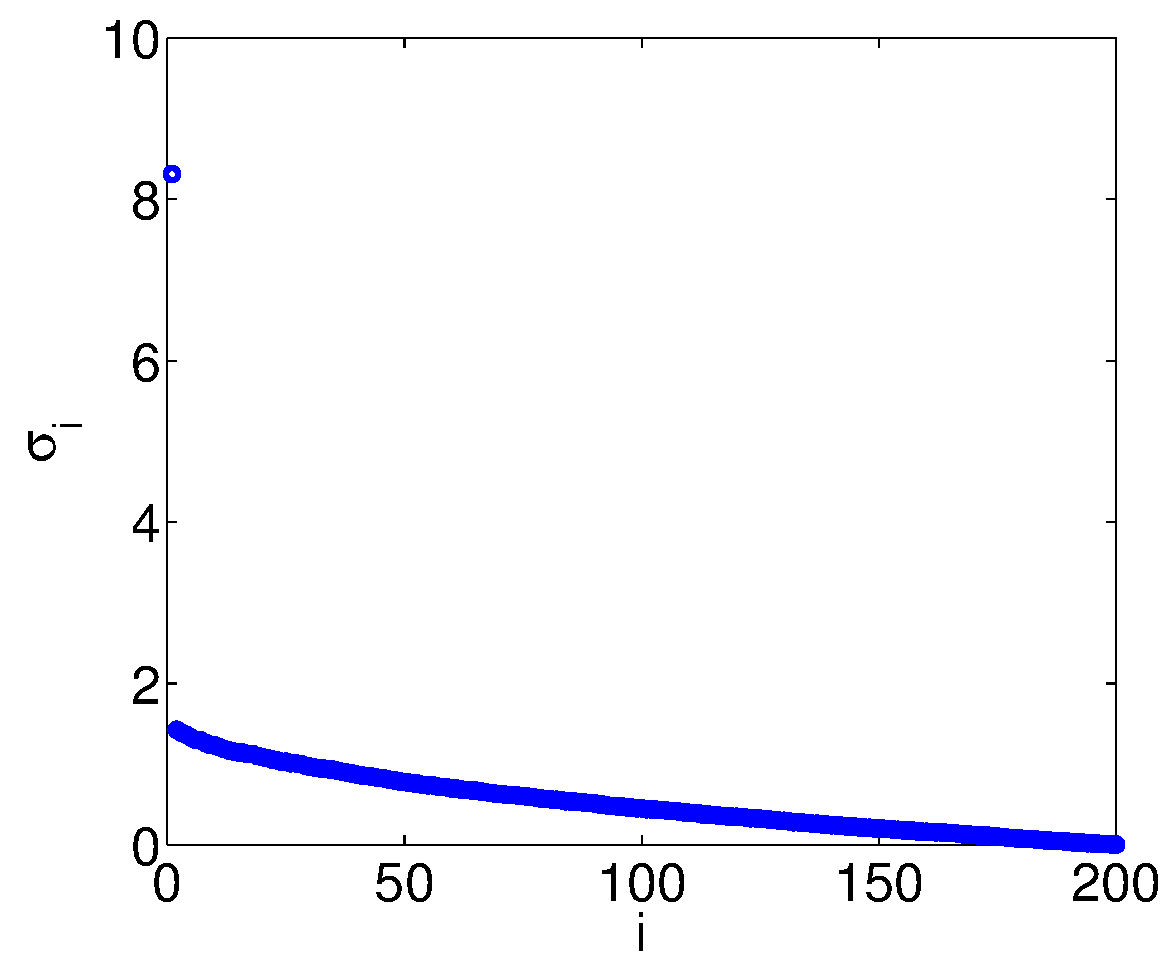
\includegraphics[width=0.4\textwidth]{chpt6_xy/figures/xy_motiv_1.pdf}
  }
  \subfigure[$\rho=0.5$, $\theta=4$]{
    \label{fig:chpt6:motiv_2}
    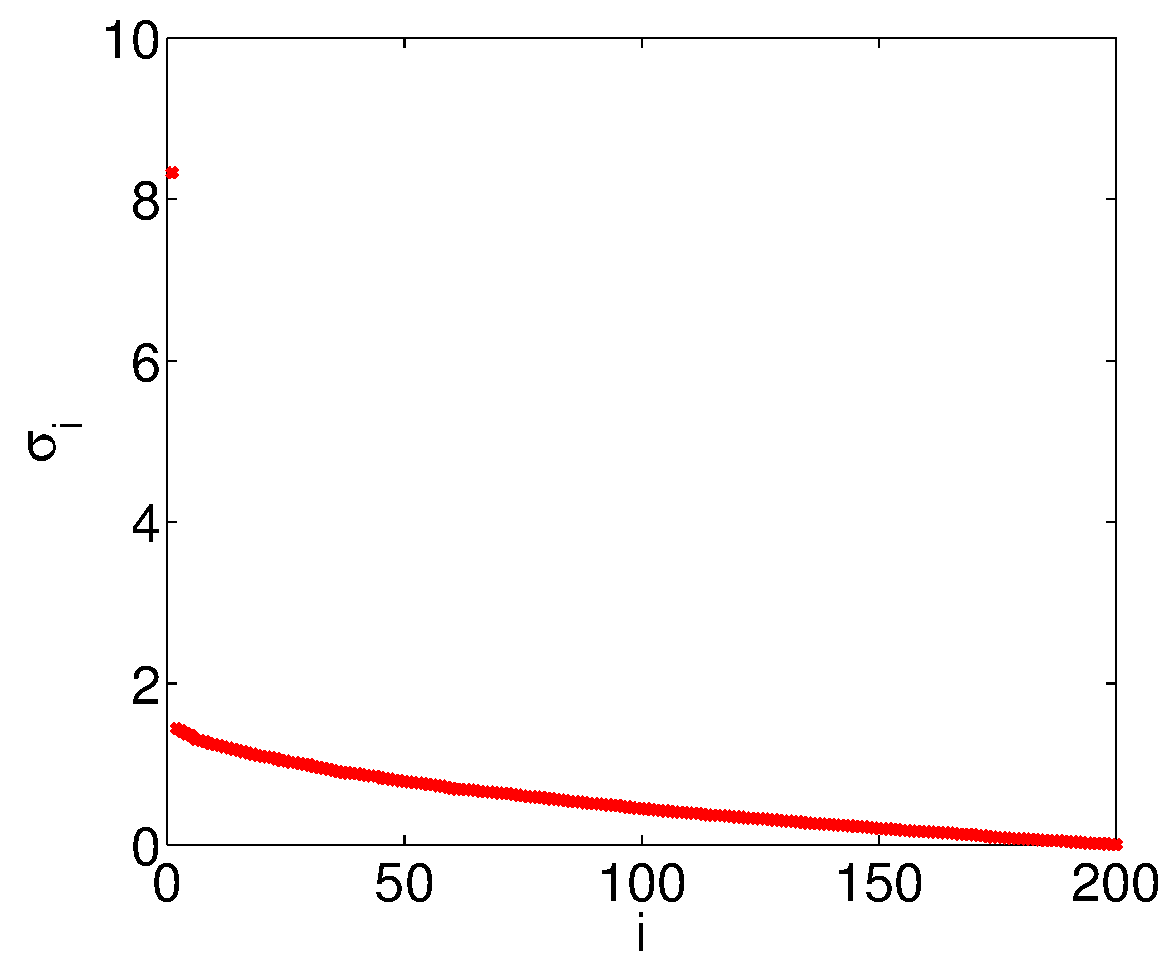
\includegraphics[width=0.4\textwidth]{chpt6_xy/figures/xy_motiv_2.pdf}
  }
  \subfigure[$\rho=0$, $\theta=10$]{
    \label{fig:chpt6:motiv_3}
   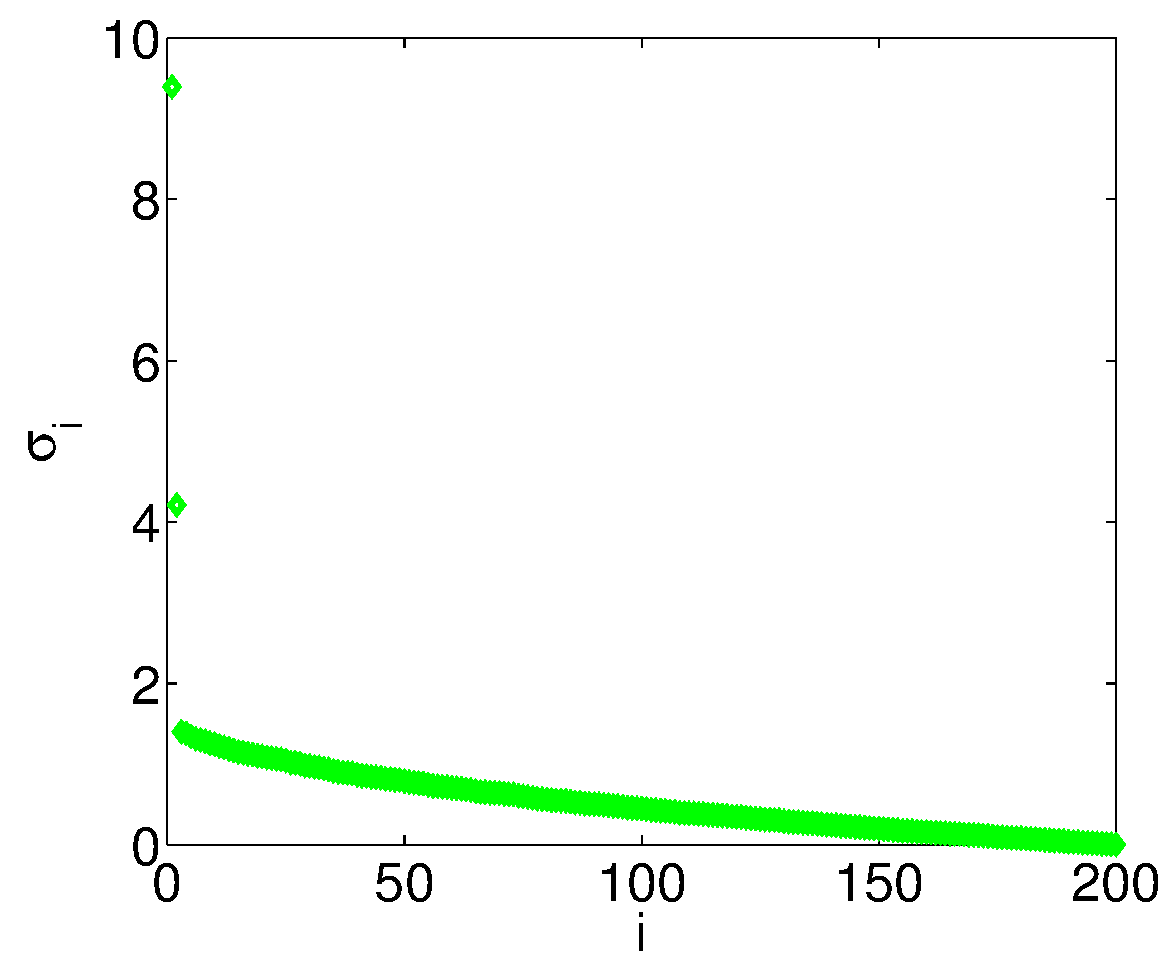
\includegraphics[width=0.4\textwidth]{chpt6_xy/figures/xy_motiv_3.pdf}
  }
  \subfigure[Combined]{
    \label{fig:chpt6:motiv_all}
    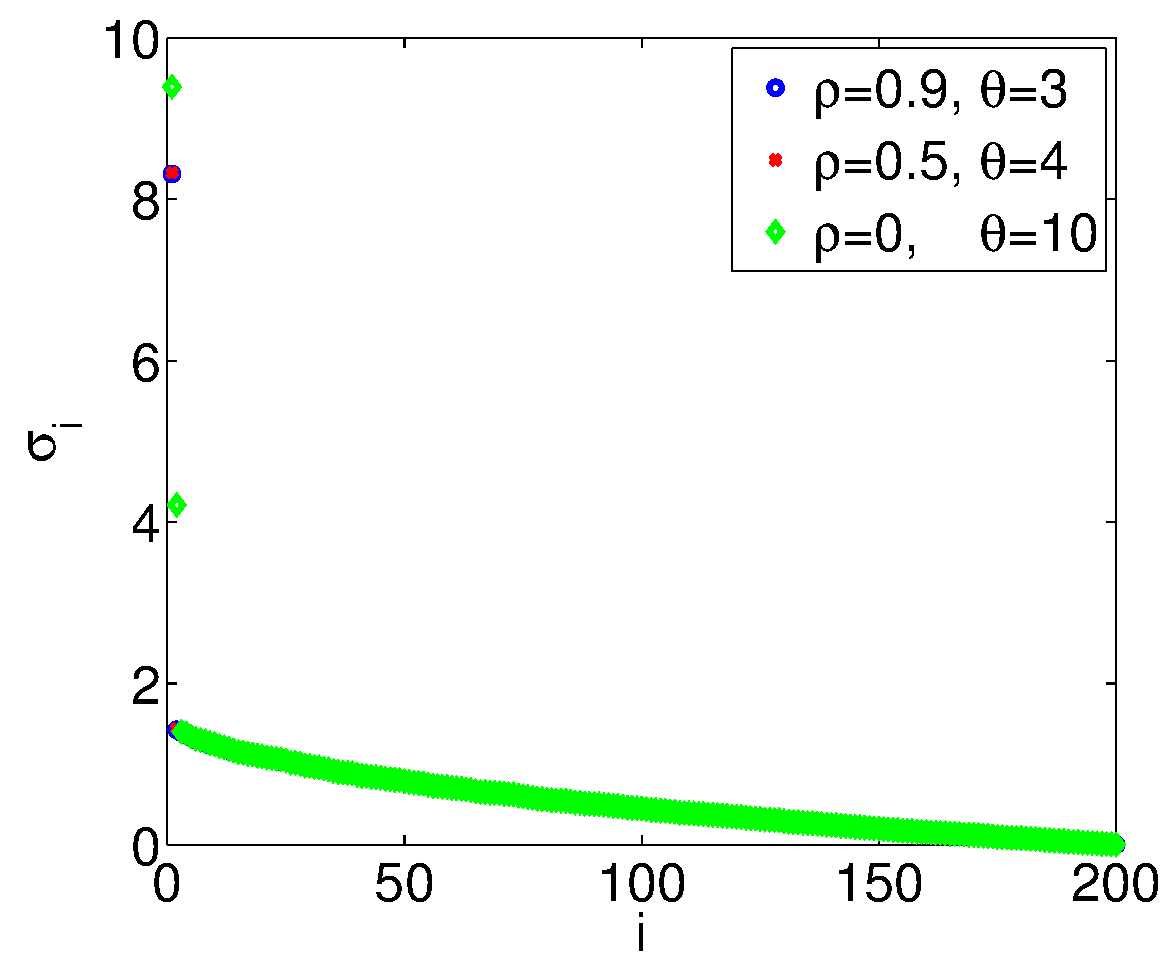
\includegraphics[width=0.4\textwidth]{chpt6_xy/figures/xy_motiv_all.pdf}
  }
  \caption{Motivational example of the singular value spectra of $\frac{1}{n}XY^H$ for three different sets of parameters. In all figures $p=q=200$, $n=500$, and $\theta=\theta_x=\theta_y$. In the settings in (a) and (b), the singular value spectra are very similar, with one singular value separating from the bulk of the singular values. In the setting in (c) where there is no correlation between the datasets, two singular values separate from the bulk of the singular values.}
  \label{fig:chpt6:motiv}
\end{figure}
